\documentclass[10pt,letterpaper]{article} 
\usepackage{toolsper}
%\usepackage{graphicx}‎‎
%\usefonttheme{serif}‎
%\usepackage{ptext}‎
\usepackage{xepersian}
\settextfont{B Nazanin}
\usepackage{lipsum}
\setlength{\parindent}{0pt}
\newcommand{\pf}{$\blacksquare$}
\newcommand{\pic}[2]{
\begin{center}
\includegraphics[width=#2]{#1}
\end{center}
}
\begin{document}
\Large
\begin{center}
به نام خدا

پاسخ تمرینات سری پنجم درس آمار و احتمال
\hl
\end{center}
سوال 1) الف)
\qn{
\Pr\{
\text{\rl{
ظاهر شدن عدد 3
}}
\}
&=
\Pr\{
\text{\rl{
ظاهر شدن عدد 3
}}
|
\text{\rl{
پرتاب دو تاس
}}
\}
\Pr\{
\text{\rl{
پرتاب دو تاس
}}
\}
\\&+
\Pr\{
\text{\rl{
ظاهر شدن عدد 3
}}
|
\text{\rl{
پرتاب یک تاس
}}
\}\Pr\{
\text{\rl{
پرتاب یک تاس
}}
\}
\\&=
{2\over 36}\times {1\over 2}+
{1\over 6}\times {1\over 2}
\\&=
{1\over9}
}{}
ب)
\qn{
\Pr\{
\text{\rl{
ظاهر شدن عدد 8
}}
\}
&=
\Pr\{
\text{\rl{
ظاهر شدن عدد 8
}}
|
\text{\rl{
پرتاب دو تاس
}}
\}
\Pr\{
\text{\rl{
پرتاب دو تاس
}}
\}
\\&+
\Pr\{
\text{\rl{
ظاهر شدن عدد 8
}}
|
\text{\rl{
پرتاب یک تاس
}}
\}\Pr\{
\text{\rl{
پرتاب یک تاس
}}
\}
\\&=
{5\over 36}\times {1\over 2}+
0\times {1\over 2}
\\&=
{5\over72}
}{}
سوال 2) 

الف) تابع \lr{CDF} باید در بینهایت به سمت یک میل کند. بنابراین $k=1$. شکل \lr{CDF} به صورت زیر است:
\begin{center}
\includegraphics[width=120mm]{Q2A.eps}
\end{center}
ب) تابع \lr{CDF} باید از راست پیوسته باشد؛ در نتیجه $k=1$ و در این صورت تابع مورد نظر، به فرم توزیع تجمعی در می آید.

پ) برای تایع توزیع تجمعی $F$ باید داشته باشیم:
$$
F(-\infty)=0\quad,\quad F(\infty)=1
$$
برای تابع 
$
{e^x+k\over e^x+1}
$
داریم:
$$
F(-\infty)=k\quad,\quad F(\infty)=1
$$
در نتیجه $k=0$. بنابراین تابع \lr{CDF} به صورت زیر است:
\begin{center}
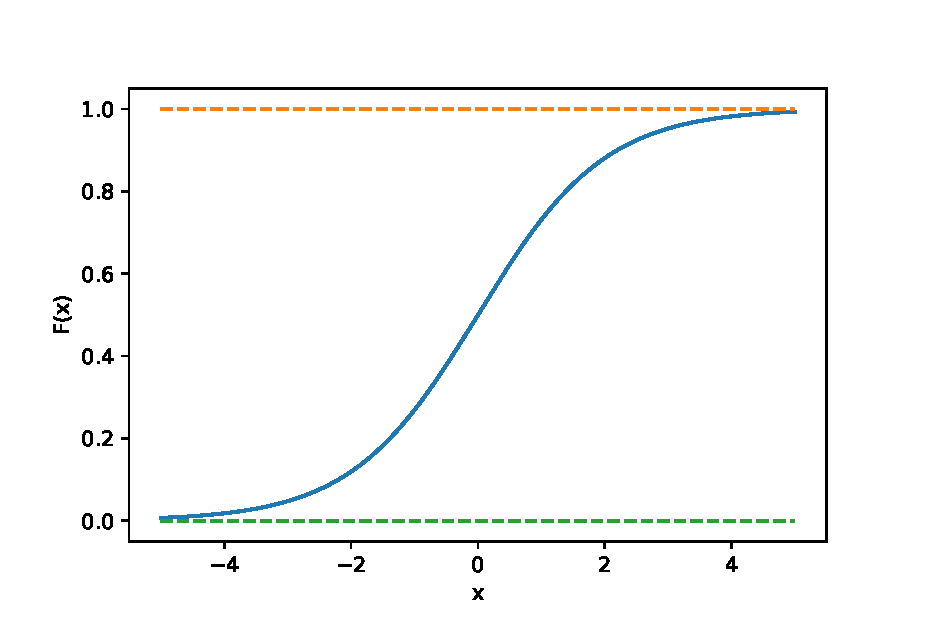
\includegraphics[width=120mm]{Q2B.eps}
\end{center}
ت) یا استدلالی مشابه قسمت قبل و با میل دادن $x$ به $+\infty$ خواهیم داشت $k=1$. در این صورت شکل تابع، به صورت زیر است:
\begin{center}
\includegraphics[width=120mm]{Q2C.eps}
\end{center}
مشاهده می شود که تابع به ازای مقادیر مثبت، مقادیر بیشتر از یک را اختیار می کند. در نتیجه تابع نمی تواند \lr{CDF} باشد.

سوال 3) طبق تعریف، میانه صدک 50 محسوب می شود و برای پیدا کردن آن، نیازمند حل معادله ی زیر هستیم:
$$
F(x)={1\over 2}
$$
 که مقدار $x=\ln2$ را برای میانه به دست می دهد.

سوال 4) طبق تعریف
$$
\Pr\{X=x\}=F(x)-F(x^-)
$$
الف)
\qn{
&F(1)={3\over 4}
\\&F(1^-)={1\over 2}
\\&\implies
\\&\Pr\{X=1\}=F(1)-F(1^-)={1\over 4}
}{}
ب)
\qn{
&F(1)={1\over 2}
\\&F(1^-)={1\over 2}
\\&\implies
\\&\Pr\{X=1\}=F(1)-F(1^-)=0
}{}
سوال 5) \lr{CDF} را با $G(x)$ و \lr{PDF} را با $g(x)$ نشان می دهیم.

الف)
\qn{
G(x)&=\Pr\{X+1\le x\}
\\&=\Pr\{X\le x-1\}
\\&=F(x-1)
}{}
در نتیجه
$$
g(x)=f(x-1)
$$
ب)
\qn{
G(x)&=\Pr\{2X\le x\}
\\&=\Pr\left\{X\le {x\over 2}\right\}
\\&=F\left({x\over 2}\right)
}{}
در نتیجه
$$
g(x)={1\over 2}f\left({x\over 2}\right)
$$
پ)
\qn{
G(x)&=\Pr\{-X\le x\}
\\&=\Pr\left\{X\ge -x\right\}
\\&=1-\Pr\left\{X< -x\right\}
\\&=1-\Pr\left\{X\le-x\right\}+\Pr\left\{X=-x\right\}
\\&=1-F(-x)+\Pr\left\{X=-x\right\}
}{}
بنابراین
$$
g(x)=f(-x)+{d\over dx}\Pr\left\{X=-x\right\}
$$
جمله ی ${d\over dx}\Pr\left\{X=-x\right\}$ شامل مشتق تابع توزیع تجمعی در ناپیوستگی هاست.

ت)
\qn{
G(x)&=\Pr\{X^2\le x\}
\\&=\Pr\left\{-\sqrt x\le X\le \sqrt x\right\}
\\&=\Pr\left\{X\le \sqrt x\right\}-\Pr\left\{X<-\sqrt x\right\}
\\&=\Pr\left\{X\le \sqrt x\right\}-\Pr\left\{X\le-\sqrt x\right\}
\\&+\Pr\left\{X=-\sqrt x\right\}
\\&=F(\sqrt x)-F(-\sqrt x)+\Pr\left\{X=-\sqrt x\right\}
}{}
که از روی آن می توان \lr{PDF} را به صورت زیر به دست آورد:
$$
g(x)={1\over 2\sqrt x}\left[f(\sqrt x)+f(-\sqrt x)\right]+{d\over dx}\Pr\left\{X=-\sqrt x\right\}
$$
سوال 6)

الف) خودروها زمانی بدون مشکل از بزرگراه رد می شوند که هر 9 تای آنها بخواهند رد شوند. این احتمال برابر $p^9$ است؛ لذا احتمال مطلوب برابر $1-p^9$ خواهد بود.

ب) 
$$
1-p^9<0.002\implies p\gtrapprox 0.9998
$$
سوال 7) قضیه ی دوموآو-لاپلاس بیان می دارد:
\qn{
\binom{n}{k}p^k(1-p)^{n-k}\approx G\left({k-np\over\sqrt{np(1-p)}}\right)
}{}
زمانی که $k$ بسیار به $n$ نزدیک و $n$ بسیار بزرگ باشد. از جمله نتایجی که می توان از این قضیه گرفت، عبارتست از:
\qn{
\sum_{k=k_1}^{k_2}\binom{n}{k}p^k(1-p)^{n-k}\approx
G\left({k_2-np\over\sqrt{np(1-p)}}\right)
-
G\left({k_1-np\over\sqrt{np(1-p)}}\right)
}{}
در این سوال:
$$
p={1\over 2}
$$
بنابراین
\qn{
\Pr\left\{0.49\le{k\over n}\le0.51\right\}&=
\sum_{0.49n}^{0.51n}\binom{n}{k}p^k(1-p)^{n-k}
\\&\approx
G\left({0.01n\over\sqrt{n\over 4}}\right)
-
G\left({-0.01n\over\sqrt{n\over 4}}\right)
\\&=
2G\left({0.02\sqrt n}\right)-1
\\&>0.95
}{}
در نتیجه
$$
G\left({0.02\sqrt n}\right)>0.975
$$
\end{document}